\documentclass[t]{beamer}


% Appearance:

\usetheme{KTHprofile}
\usefonttheme[onlylarge]{structurebold}



% Standard packages

\usepackage[english]{babel}
\usepackage[latin1]{inputenc}
\usepackage{times}
\usepackage[T1]{fontenc}
\usepackage{lipsum}
\usepackage[]{epstopdf}
% Author, Title, etc.

%\title{}

\title[Inisintiur sequi aliquia tis dis in para] 
{%
  Safe Learning for Control%
}

%\author{}

\author[Oskar, Friends]
{
Caroline Heidenreich
}

%\author[Dude, Friends]
%{
%The~Dude\inst{1} \and
%And~Friends\inst{2}
%}

\institute{}

%\institute[KTH Royal Institute of Technology]
%{\inst{1} KTH Royal Institute of Technology, Sweden\and
%\vskip-4mm
%\inst{2} KTH Royal Institute of Technology, Sweden
%}

\date{\today}


\begin{document}


\begin{frame}
\titlepage
\end{frame}


\begin{frame}
\frametitle{Contents}

\begin{itemize}
\item Motivation
\item Algorithm
\item Results
\item Conclusions and Future Work
\end{itemize}
\end{frame}

\begin{frame}
\frametitle{Motivation}
\framesubtitle{Why do we want to do safe learning in control?}
\begin{itemize}
\item model-based control suffers often from poor model accuracy
\item reinforcement learning algorithms not designed for satisfying constraints
\end{itemize}

\end{frame}


\begin{frame}
\frametitle{Algorithm}
\framesubtitle{How to we do safe learning for control?}
Example
\begin{itemize}
\item autonomous vehicle with partly known model
\item task: learn control without driving off the road
\end{itemize}

\begin{figure}[h!]
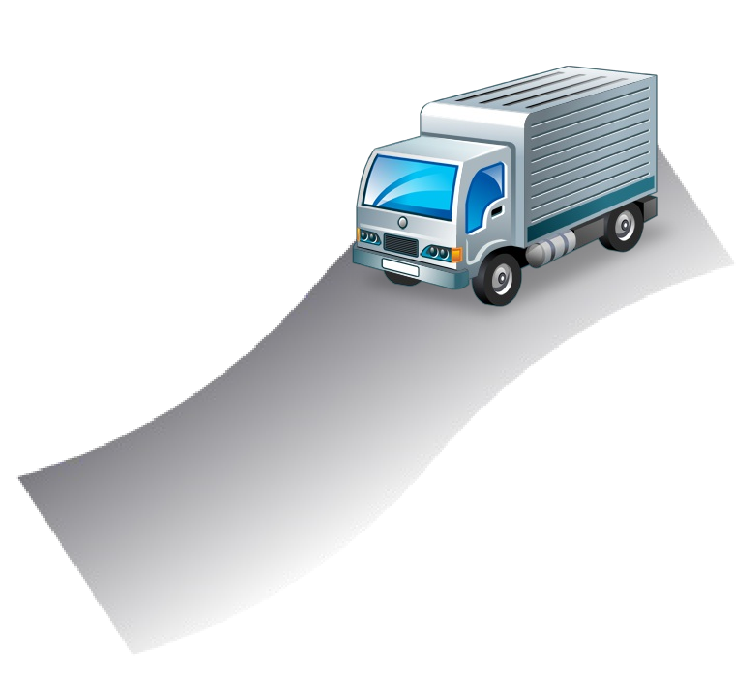
\includegraphics[width=0.4\paperwidth]{TruckOnStreet}
\caption{The truck}
\end{figure}


\end{frame}

\begin{frame}
\frametitle{Algorithm}
\framesubtitle{Reinforcement Learning}
General Idea: Finding the optimal policy by trying actions and receiving rewards
\begin{itemize}
\item 
\end{itemize}

\begin{figure}[h!]
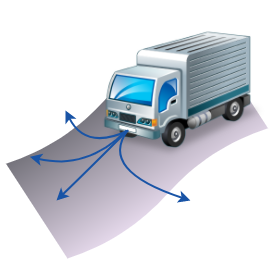
\includegraphics[trim=0mm 0mm 0mm 0mm, width=0.4\paperwidth]{PossibleTrajectories}
\caption{Possible Trajectories}
\end{figure}


\end{frame}


\begin{frame}
\frametitle{Algorithm}
\framesubtitle{Safe Set Calculation}
\begin{itemize}
\item 
\end{itemize}
\end{frame}


\begin{frame}
\frametitle{Algorithm}
\framesubtitle{Disturbance Estimation with Gaussian Processes}
\begin{itemize}
\item 
\end{itemize}
\end{frame}

\begin{frame}
\frametitle{Algorithm}
\framesubtitle{Exploration}
\end{frame}

\begin{frame}
\frametitle{Experimental Results}
\framesubtitle{Policy Estimation}
\begin{itemize}
\item 
\end{itemize}
\end{frame}

\begin{frame}
\frametitle{Experimental Results}
\framesubtitle{Disturbance Estimation}
\begin{itemize}
\item 
\end{itemize}
\end{frame}

\begin{frame}
\frametitle{Experimental Results}
\framesubtitle{Simulation}
\begin{itemize}
\item 
\end{itemize}
\end{frame}


\begin{frame}
\frametitle{Conclusions}
\begin{itemize}
\item 
\end{itemize}
\end{frame}

\begin{frame}
\frametitle{Future Work}
\begin{itemize}
\item 
\end{itemize}
\end{frame}
\end{document}